\documentclass[11pt, a4paper]{article} %or article has only section and below, book and report also have chapter: http://texblog.org/2007/07/09/documentclassbook-report-article-or-letter/

\usepackage[utf8]{inputenc}  % use utf8 encoding of symbols such as umlaute for maximal compatibility across platforms

\usepackage{caption}      	% provides commands for handling caption sizes etc.
%\usepackage[a4paper, left=25mm, right=20mm, top=25mm, bottom=20mm]{geometry}		 % to easily change margin widths: https://www.sharelatex.com/learn/Page_size_and_margins

\usepackage{etoolbox}    % for conditional evaluations!
%\usepackage{fancyverb}   % for syntax highlighting of R code, together with the listings package
\usepackage[bottom]{footmisc}  % I love footnotes! And they should be down at the bottom of the page!
\usepackage{graphicx}        % when using figures and alike
\usepackage[hidelinks]{hyperref}		% for hyperreferences (links within the document: references, figures, tables, citations)
%\usepackage{listings}

\usepackage{euler}     % a math font, only for equations and alike; call BEFORE changing the main font; alternatives: mathptmx, fourier, 
%\usepackage{gentium} % for a different font; you can also try: cantarell, charter, libertine, gentium, bera, ... http://tex.stackexchange.com/questions/59403/what-font-packages-are-installed-in-tex-live

%------------------------------------------------------------------------------------------------------
%------- text size settings --------------
\setlength{\textwidth}{16cm}% 
\setlength{\textheight}{25cm} %23 
%(these values were used to fill the page more fully and thus reduce the number of pages!)
\setlength{\topmargin}{-1.5cm} %0
\setlength{\footskip}{1cm} %
%\setlength{\hoffset}{0cm} %
\setlength{\oddsidemargin}{1cm}%
\setlength{\evensidemargin}{-.5cm}%
\setlength{\parskip}{0cm} % Abstand zwischen Absätzen
% ----------------------------------------------------------------
\renewcommand{\textfraction}{0.1} % allows more space to graphics in float
\renewcommand{\topfraction}{0.85}
%\renewcommand{\bottomfraction}{0.65}
\renewcommand{\floatpagefraction}{0.70}


\frenchspacing %http://texwelt.de/wissen/fragen/1154/was-ist-french-spacing-was-macht-frenchspacing
%------------------------------------------------------------------------------------------------------
%------------------------------------------------------------------------------------------------------

\usepackage{Sweave}
\begin{document}
\Sconcordance{concordance:newsweave.tex:newsweave.Rnw:%
1 39 1 1 0 21 1 1 9 5 1 1 7 1 2 9 1 2 2 7 1 1 5 1 1 1 7 1 2 15 0 1 2 30 %
1}



\title{Appendix}

\author{Torfinn Belbo and Carolina Wackerhagen}

\maketitle

%------------------------------------------------------------------------------------------------------
%------------------------------------------------------------------------------------------------------


\section{Introduction}%------------------------------------------------------------------------------------------------------

We created an appendix of meta-analysis paper. To be able to visualize the output, we used an example dataset taken from Gibson et al. 2011.

%The conducted analysis using the function rma from the metafor pacakge should be renamed as such: rma of a random effects model should be named ``rma.RE'' and an rma of a fixed effects model should be named ``rma.FE'' in order for the automatisation to work. IF a meta-regression has been conducted, it should be called ``rma.RE.meta'' or ``rma.FE.meta'' respectively. Other than that, the metafor package in R needs to be installed.  \\

% You should save your rma analysis and the meta regression analysis as an R object and then load it into this script in the preceeding chunk.



%Here a forest plot is created with the information from the rma.RE 
\begin{figure}
\captionsetup{width=0.6\textwidth}
\centering
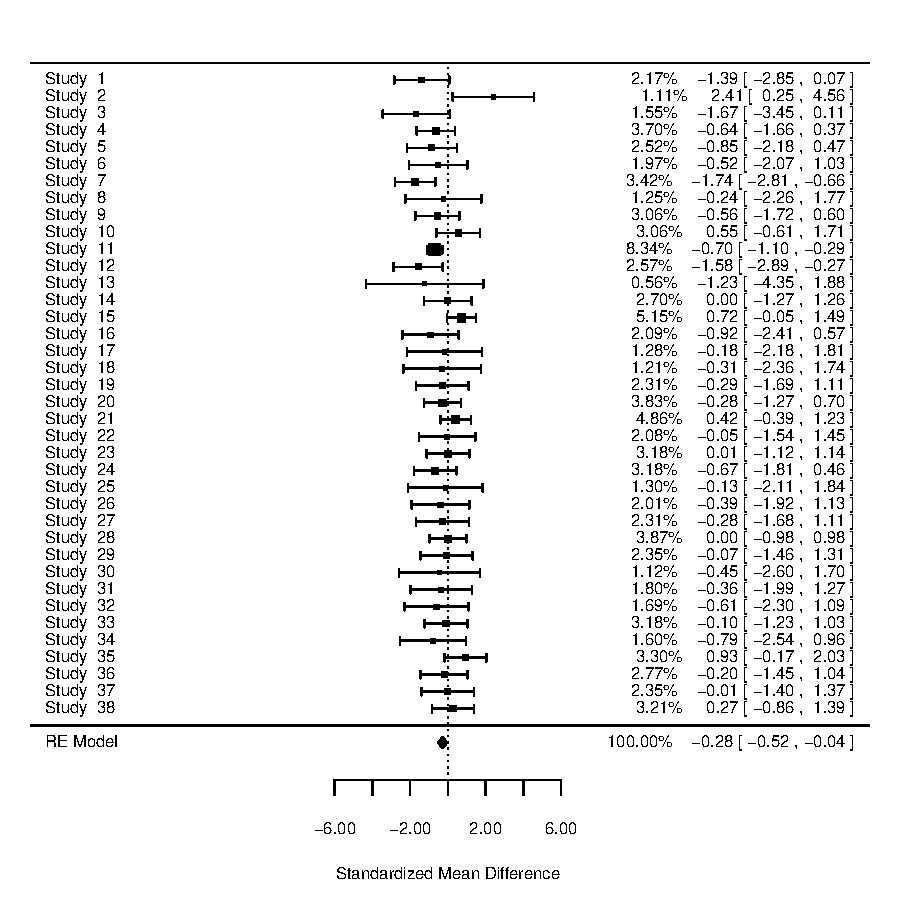
\includegraphics{newsweave-forest_re}

\caption{Forest plot of a random effects model. The column on the left represents the studies used in the meta-analysis. The weighted percentage is shown as well as the effect size (ES) [+- 95\% CI]}
\end{figure}


To assess possible publication bias, funnel plots can be used for visualization purposes.\\

\begin{figure} 
\captionsetup{width = 0.6\textwidth}
\centering
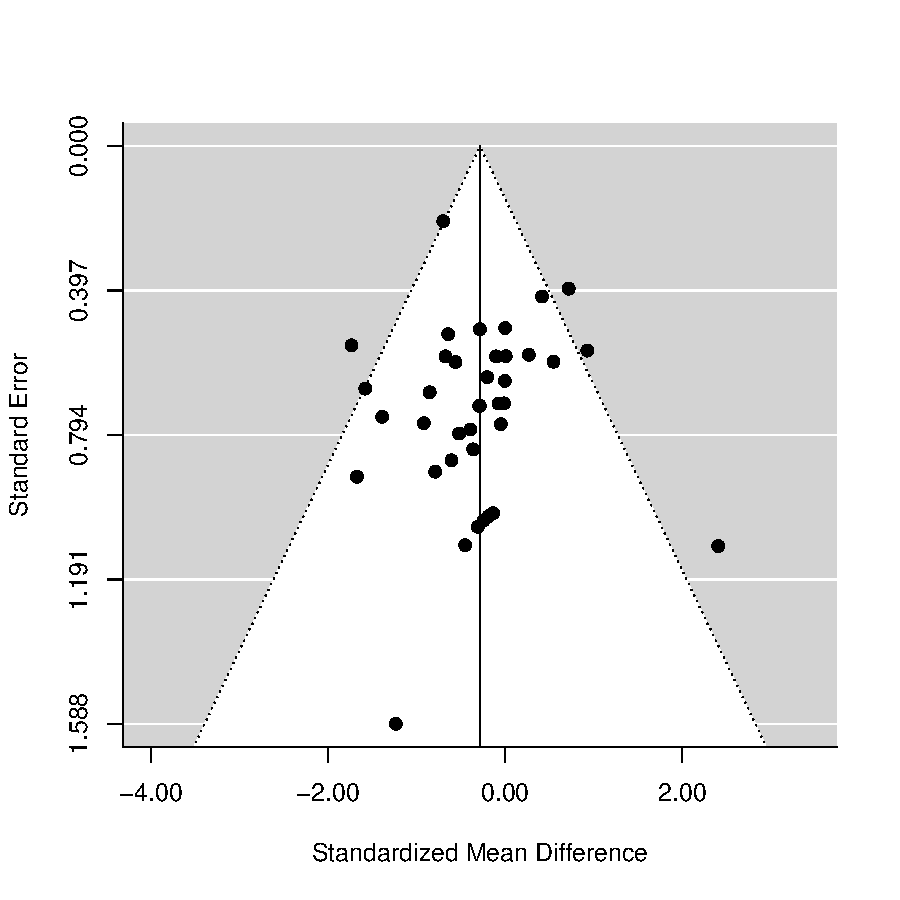
\includegraphics{newsweave-funnelplot}
\caption{Funnel plot of random effects model displaying possible publication bias. The true ES is displayed by the solid verical line.}
\end{figure}


%Table with values for ES, SE (ES),pES, CI, I2, Egger value and fasil-sage number. If various rma analysis are run, they can be loaded into this table as well. 
?? How can a an automised table be created for rows from e.g. different rma objects? In our case, we just have one rma object so one row is produced. If the people conduct different rmas for different data subsets, it would be nice to have this in the same table as well!\\
\bigskip




% latex table generated in R 3.1.2 by xtable 1.7-4 package
% Sun Nov 23 17:59:11 2014
\begin{table}[ht]
\centering
\caption{Results of the meta-analysis. Includes the the egger's test and the fails-safe number for publication bias testing} 
{\footnotesize
\scalebox{0.9}{
\begin{tabular}{rrrrrrrrrrrr}
  \hline
 & Effect.Size & SE.of.Effect.Size & CI..lb. & CI.ub. & P.ES. & Q & P.Q. & I.2 & Egger & P.Egger. & FSN \\ 
  \hline
Value & -0.28 & 0.12 & -0.52 & -0.04 & 0.02 & 47.05 & 0.12 & 27.22 & -0.44 & 0.66 & 77.00 \\ 
   \hline
\end{tabular}
}
}
\end{table}\bigskip



This table should work once you have saved the rma.RE.meta and loaded it at the top of the document!!! Take it out of the \% \\

%<<echo = FALSE, eval = TRUE>>=
%matrix.RE.meta = data.frame(t(c("Effect Size"=rma.RE.meta$b, "SE of Effect Size"=rma.RE.meta$se, "CI (lb)"= rma.RE.meta$ci.lb, "CI(ub)" = rma.RE.meta$ci.ub, "P(ES)" = rma.RE.meta$pval, "Q" = rma.RE.meta$QE, "P(Q)" = rma.RE.meta$QEp, "I^2" = rma.RE.meta$I2, "Test of Moderators" = rma.RE.meta$QM, "P(Moderator Test)" = rma.RE.meta$QMp)))
%rownames(matrix.RE) <- "Africa", "Asia", "Central America", "South America"
%require(xtable)
%mytable2 = matrix.RE.meta
%@

%<<xtable2, results = tex, echo=FALSE>>=
%print(xtable(mytable2, caption = paste("Results of the meta-regression. Test for heterogeneity taking all four continents into account")),caption.placement = "top", size ="footnotesize", scalebox = 0.9)
%@

To do:

Add a table with the results from the meta regression + add a bubble plot. Add the 4 figures as well and a table for the sensitivity analysis. 

!!! I tried saving the rma.meta.RE as an object but I encountered problems with saving it, as it said it cannot open the compressed file. Haven't found a solution till now. Maybe you can save the object? :)

Do the same for the meta package or use the forest plot from the meta package\\

Notes:

Are we going to make two scripts? One for meta and one for metafor or are we going to do a combination? Plus write a function for this script? 
Don't know if this such a good idea as the appendix is not that good. Especially the table. Till now it would only work with one rma.RE object with one row and not many. Is is possible to combine specific single values of various rma objects? Can we do this?

\end{document}
